% Author: Pavol Loffay
% Project: Master thesis - Hawkular alert prediction
% Date 20.2.2015

\chapter{Introduction}
In driving successful business on the internet it is important to assure an application
health and reliability. One can achieve that by monitoring subjected resources and setting
up a clever alerting system. These features are offered in many monitoring systems, however 
being predictive in this area can even prevent undesirable states and most importantly gives administrators more time for
reacting to such events. For instance it can decrease downtime of an application 
or ability to load balance workload in advance by horizontal scaling targeted services. 

As alerting system are sophisticated and can be composed by many conditions so this work
focuses only on predicting future metrics values which are then sent as input to an alerting system. 

In the first chapter are discussed various approaches for time series modeling and
forecasting. Second chapter focuses on implemented models with validation on real and 
generated test data sets. Implementation details with testing can be found in fourth chapter.

TODO describe chapters

    \section{Hawkular}
    The implementation part of the master's thesis is developed as a part of an open source project
    Hawkular\footnote{Available at \url{http://www.hawkular.org}}. 
    Therefore the application architecture and used technologies had to fit 
    into the overall project architecture.

    Hawkular is middleware monitoring and management platform
    developed by company Red Hat and independent community of contributors.
    It is a successor to very successful RHQ\footnote{Available at \url{https://rhq-project.github.io/rhq/}} 
    project, also known as JBoss Operations Network.
    By monitoring is meant that there are agents for diverse applications which
    push data to the server. These agents can also execute application specific actions. 

    The monolithic architecture of RHQ project was due it's size hard to maintain 
    and lacking robust REST API lead to fresh development of new application.   
    In contrast Hawkular consist of several loosely coupled or even independent applications.
    These independent components are much
    easier to maintain and more importantly they communicate over REST API. This
    architecture of microservices and chosen protocol allow simple development of 
    agents which can be written in any programming language. In RHQ only Java agent were
    available. Hawkular as product is customized Wildfly
    \footnote{An open source project of JBoss EnterpriseApplication Platform.}
    application server with all components deployed in it.

    \begin{itemize}
        \item Console\,--\,user web interface
        \item Accounts\,--\,authorization subsystem based on Keycloak\footnote{An open
            source single sing-on and identity management for RESTful web services.}
        \item Inventory\,--\,graph based registry of all entities in Hawkular
        \item Metrics\,--\,time series metrics engine based on Cassandra\footnote{An open
            source distributed database management system. Hybrid between key\,--\,value and
        column\,--\,oriented database.}
        \item Alerts\,--\,alerting subsystem based on JBoss Drools
    \end{itemize}

    Some of the modules uses also Java messaging topics (JMS) for inter\,--\,component
    one to many communication.

    Modules are packaged as standard Java web archives (WAR), or enterprise archives (EAR)
    and deployed into customized Wildfly. Build and package management is performed by 
    Maven and Gulp for user interface modules. 

    \section{Data Mining Goals}
    The goal of this thesis is to develop module for Hawkular which will provide forecasts for any 
    time series metrics collected by agent. On new metric data available the module
    learns from data and predicts new values. Based on this predicted values an alert can
    be triggered. Forecast should be also available for user interface in predictive
    charts. 

    One Wildfly agent on average collects hundreds to thousands metrics, therefore module
    should be capable of processing high volume of data. Some of the customers monitor
    hundreds of server each with multiple agents. Therefore performance of chosen 
    learning algorithm has to be taken in account.

%%%%%%%%%%%%%%%%%%%%%%%%%%%%%%%%%%%%%%%%%%%%%%%%%%%%%%%%%%%%%%%%%%% 
\chapter{Existing Solutions}
%TODO
TODO describe existing software.


%%%%%%%%%%%%%%%%%%%%%%%%%%%%%%%%%%%%%%%%%%%%%%%%%%%%%%%%%%%%%%%%%%% 
\chapter{Time Series Models}
This chapter focuses on time series theory and various approaches for modelling time series.
Models are ordered from simpler to more complex ones. 

Firstly, it is important to define time series; it is sequence of observations
$s_t \in \mathbb{R}$ ordered in time. This thesis focuses only on univariate equidistant 
discrete time series. Time series analysis contains many segments, this work focuses on 
forecasting. It is defined as a process of making prediction of the future based 
on the past. In other words, forecasting is possible because  
future depends on the past or analogously because there is a relationship
between the future and the past. However, this relation is not deterministic and 
can be hardly written in an analytical form.

There are two forecasting types: qualitative and quantitative.
Qualitative methods are mainly based on the opinion of the subject and are used 
when past data are not available, hence not suitable for this project. 
If there are past data available, quantitative forecasting methods are more suitable. 

    %%%%%%%%
    \section{Simple quantitative methods}
    Following methods are the simples forecasting quantitative models. They can be used on
    any time series without further analysis. 

    \begin{itemize}
        \item Average method\,--\,forecasts are equal to the value of the mean of
            historical data.
            \begin{eqnarray}
                \hat{y}_{T+h|T} = \overline{y} = (y_{1}+ \dots + y_{T}) / T 
            \end{eqnarray}
        \item Na\"{i}ve method\,--\,forecasts are equal to the last observed value.
            \begin{eqnarray}
                \hat{y}_{T+h|T} = y_{T}
            \end{eqnarray}
        \item Drift method\,--\,variation of na\"{i}ve method which allow the
            forecasts to increase or decrease over time.
            \begin{eqnarray}
                \hat{y}_{T+h|T} = y_{T} + \frac{h}{T-1} \sum_{t=2}^T{y_{t} - y_{t-1}} = 
                    y_{T} + h(\frac{y_{T}-y_{1}}{T-1}) 
            \end{eqnarray}

    \end{itemize}
    There is also a seasonal variant of na\"{i}ve model. This method is suitable only
    for highly seasonal data. These methods in general produces high forecasting error 
    but are very easy to implement.

    %%%%%%%%
    \section{Linear Regression}
    Linear regression is classical statistical analysis technique. It is often used to
    determine whether there is linear relationship between dependent and eventually more
    independent variables. It is also often used for predictions mainly in econometric
    field. 

    Simple linear regression is defined as:
    \begin{eqnarray}
        y = \beta_0 + \beta_1 x + \epsilon
    \end{eqnarray}

    Parameters $\beta_0$ and $\beta_1$ are calculated by minimizing the sum of squared
    errors:
    
    \begin{eqnarray}
        SSE = \sum_{i=1}^N \epsilon_{i}^2 = \sum_{i=1}^N (y_i - \beta_0 - \beta_1 x_i)^2
    \end{eqnarray}
    
    Once parameters are estimated predictions for any time in the future can be calculated. 
    If modelled time series is not stationary then and for instance trend changes over
    time parameters has to be periodically estimated to achieve better accuracy. 
    %For econometric analysis it is important to use best linear unbiased estimator,
    %where couple of assumptions has to hold:
    %\begin{enumerate}
    %    \item $E(Y_i) = \beta_0 + \beta_1 X_i$
    %    \item $var(Y_i)=\sigma^2$\,--\,homoscedasticity
    %    \item $cov(Y_i, Y_j)=0$, for $i \neq j$
    %    \item $Y_i$ cames from normal distribution
    %    \item $X_i$ is not random variable
    %\end{enumerate}
    %Where $i$ takes values from $1$ to the number of observed values. These assumptions 

    %%%%%%%%
    \section{Simple Exponential Smoothing}
    The concept behind simple exponential smoothing is to attach 
    larger weights to the most recent observations than to observations from distant
    past. Forecasts are calculated using weighted averages where the weights 
    decrease exponentially as observations come from further in the past.
    In other words smaller weights are associated to older observations.
    Equation for simple exponential smoothing is listed in \ref{exp_smoothing}.

    \begin{eqnarray} \label{exp_smoothing}
         \hat{y}_{T+1|T} = l_t \\ \nonumber
         l_t = \alpha y_t + (1-\alpha)l_{t-1}
    \end{eqnarray}

    For smoothing parameter $\alpha$ holds $ 0 \leq \alpha \leq 1 $. Note, if $\alpha = 1$ then \\
    $\hat{y}_{T+1|T} = y_{T}$ so forecasts are equal to the na\"{i}ve method.
    If the parameter $\alpha $ is smaller more weight is given to observations from distance
    in past. 

    Simple exponential smoothing has flat forecast function, that means all forecasts
    all the same. Smoothing can be generally used as technique to separate signal and noise.
    This method is useful if a series does not contain any trend or one is interested only
    in one step ahead prediction. Multi step ahead predictions for time series with trend
    can produce high error.

    %%%%%%%%
    \section{Holt's Liner Trend Method}
    Simple exponential smoothing can be extended to allow forecasting of data with a trend. 
    This was done by Charles C. Holt in 1957. This method is slightly more complicated than 
    original one without trend. In order to add trend component another equation has to be added. 

    \begin{eqnarray} \label{exp_holt}
        \hat{y}_{t+h|t} = l_{t} + hb_{t} \\ \nonumber
         l_t = \alpha y_t + (1 - \alpha) (l_{t-1} + b_{t-1}) \\ \nonumber
         b_t = \beta (l_t - l_{t-1}) + (1 - \beta)b_{t-1} 
    \end{eqnarray}

    Where a parameter $b_t$ denotes a slope of the series and the parameter $l_t$ level. 
    There is also a new parameter smoothing parameter of the slope\,--\,$\beta$. 
    It's rage is equal to $\alpha$, so $\alpha,\beta \in \interval[{0,1}]$. 

    %%%%%%%%
    \section{Holt\,--\,Winters Seasonal Method}
    This method is an extension of Holt's linear trend method with added
    seasonality. It is also called triple exponential smoothing. In this model 
    there are three equations \ref{exp_holt_winters}. 
    One for level, second for trend and third for seasonality.
    Each pattern uses smoothing constant $ \alpha,\beta,\gamma \in \interval[{0,1}]$.

    \begin{eqnarray} \label{exp_holt_winters}
        \hat{y}_{t+h|t} = l_{t} + hb_{t} + s_{t+h_m-m}\\ \nonumber
        l_t = \alpha (y_t - s_{t-m}) + (1 - \alpha) (l_{t-1} + b_{t-1}) \\ \nonumber
        b_t = \beta (l_t - l_{t-1}) + (1 - \beta)b_{t-1} \\ \nonumber
        s_t = \gamma (y_t - l_{t-1} - b_{t-1}) + (1-\gamma)s_{t-m}
    \end{eqnarray}

    Where $h_m=[(h-1) \mod m] + 1$, which ensures that the estimates of the seasonal
    indices came from the correct season. This model can be used only if the period 
    of time series is know beforehand. In Hawkular the period of the time series is 
    unknown, therefore period identification should be also implemented.
    
    %%%%%%%%
    \section{Time series decomposition}
    Many models decompose time series and then model it without these patterns
    \cite{otexts}. One example of such a model is ARIMA.
    Basic observed patterns are trend, seasonality, cycle and irregular
    component often called called white noise. 
    
    \begin{itemize}
        \item \textbf{Trend $ T_{t} $}\,--\,exists if there is long term increase or decrease over
            time. Can be linear or nonlinear (e.g. exponential growth)
        \item \textbf{Seasonal $ S_{t} $}\,--\,exists when a series is influenced by seasonal factors.
            Seasonality is always of fixed and known period.
        \item \textbf{Cyclic $ C_{t} $}\,--\,exists it there are long term wave-like patterns.
            Waves are not of a fixed period.
        \item \textbf{Irregular $ N_{t} $}\,--\,unpredictable random value referred as white
            noise. 
    \end{itemize}

    Decomposition can be written in many forms. Two of them are additive and
    multiplicative form.

    \begin{eqnarray}
        y_{t} = T_{t} + S_{t} + C_{t} + N_{t} \\
        y_{t} = T_{t} \times S_{t} \times C_{t} \times N_{t} 
    \end{eqnarray}

    In the following sections are discussed time series models for which is decomposition
    crucial.

    %%%%%%%%
    \section{Box\,--\,Jenkins Methodology (ARIMA)}
    Methods from Box\,--\,Jenkins methodology are the most widely used in time series
    modelling specially for econometric data. It analyzes autocorrelations (ACF) and partial autocorrelations (PACF) between lagged
    observations. Outcome of these two functions can be used to estimate an order of the
    model \cite{cipra}. 

    The most used model is $ARIMA(p, d, q)$. It combines autoregressive, integrated and
    moving average. Autoregressive model consist of sum of weighed lagged values.
    The order of this model is identified by $p$. Parameters can by estimated by ordinary
    least squares method \cite{brockwell}. In other words all historical data are 
    necessary for parameters estimation. For stationary time series it converges to the mean 
    of the time series . An autoregressive model of order $p$ is written in \ref{ar_model}.

    \begin{eqnarray} \label{ar_model}
        y_t = c + e_t + \phi_1 y_{t-1} + \phi_2 y_{t-2} + \dots + \phi_p y_{t-p} \\ \nonumber
        e_t \overset{iid}{\sim} N(0, \sigma^2)
    \end{eqnarray}

    Next part of an ARIMA model is moving averages. It should not be confused with simple moving 
    average which is used for a trend estimating. In moving average model $MA(q)$ a current value is 
    a regression against white noise of prior values of the series. A random noise from 
    each point is assumed to come from the same distribution which typically is 
    a normal distribution. Model of order $q$ is in \ref{ma_model}.The estimation of
    model parameters requires all points of time series. Calculations is done with 
    Yule-Walker equations \cite{brockwell}.

    \begin{eqnarray} \label{ma_model}
        y_t = c + e_t + \theta_1 e_{t-1} + \theta_2 e_{t-2} + \dots + \theta_p y_{t-q}
    \end{eqnarray}

    It is important to mention that models $AR(p)$ and $MA(q)$ are invertible. 
    Therefore any stationary $AR(p)$ model can be written as $MA(\infty)$
    \cite{brockwell}. Last part of an $ARIMA$ model is $I(d)$. It denotes 
    number of differentiations made on the original time series. Let's define 
    backshift operator $By_t=y_{t-1}$. With this operator $ARIMA(p, d, q)$ is
    written in \ref{arima}. On the left side of the equation is $AR(P)$ process 
    and on the right $MA(q)$.

    \begin{eqnarray} \label{arima}
        (1- \phi_1B - \dots - \phi_pB^p)(1-B)^d y_t = \\ \nonumber
         c + (1+\theta_1B+\dots+\theta_qB^q) e_t
    \end{eqnarray}

    %%%%%%%%
    \section{Neural Networks}
    %TODO
    TODO

    %%%%%%%%
    \section{Adaptive Filtering}
    %TODO
    TODO


%%%%%%%%%%%%%%%%%%%%%%%%%%%%%%%%%%%%%%%%%%%%%%%%%%%%%%%%%%%%%%%%%%% 
\chapter{Models on Real Data}
In the previous chapter several methods for forecasting were discussed, however
in our system only a few of them were selected and implemented. In this chapter 
will be compared models real data.

    %%%%%%%%
    \section{Metrics in Hawkular}
    In Hawkular there are three types of metrics: gauge, counter and availability. 
    All of them are univariate metrics of structure $ \{timestamp, value\} $.

    %%%%%%%%
    \section{Evaluating Forecast Accuracy}
    In order to evaluate model it is important to estimate an error of the forecast. There are 
    several methods for evaluating forecasting errors. Chosen were two MAE and RMSE. They are 
    very similar however, RMSE gives relatively high weight to larger errors.

    $$ MAE = \frac{1}{n} \sum_{i=1}^{n} |y_i - \hat{y_i}| $$
    $$ RMSE = \sqrt{\frac{1}{n} \sum_{i=1}^{n}(y_i - \hat{y_i})^2} $$

    %TODO
    TODO show all charts of all described models. 

%%%%%%%%%%%%%%%%%%%%%%%%%%%%%%%%%%%%%%%%%%%%%%%%%%%%%%%%%%%%%%%%%%% 
\chapter{Design and Implementation}
Module for an alert prediction was named Hawkular Data mining. Source
code\footnote{Available at \url{https://github.com/hawkular/hawkular-datamining}} is versioned in Git
hosted on Github. On every commit a build with integration and unit tests was triggered in
Travis CI. Pull requests were always reviewed by some team member.

In the following chapters is described integration, design and the most important
sections of implementation.

    %%%%%%%%
    \section{Integration with Hawkular}  
    Data mining module had to follow architecture of the whole Hawkular application.
    The same approach was followed as in other modules. That means the module 
    works also in standalone fashion without Hawkular. The build produces two Java
    web applications packaged as WAR. One is for standalone usage and other with
    integration code for Hawkular.

    Integration with Hawkular is showed in \ref{img_integration}.
    The module interacts with Inventory, Metrics and Alerts. User interface uses Data
    mining REST API for getting predictions for charts. Communication is done through 
    Java messaging system and REST calls. Therefore modules are
    loosely coupled.

    Metrics definitions and prediction metadata are stored in Inventory.
    Communication flows through JMS request response temporary queues. This was
    implemented specially for asking data across all tenants.

    Forecasting of 
    metrics in Hawkular is enabled by creating relationship from tenant to tenant, metric type
    or directly to metric in Inventory. Lower levels overrides higher (configuration on metric overrides
    configuration on metric type or tenant\dots). Every change in Inventory is sent to bus topic
    where other modules can consume it. When prediction gets enabled Data mining queries all
    historical metrics to initialize model.

    When Metrics receives data from Agent it sends them to topic where is consumed by Alerts
    and Data mining. If metric if being forecasting model weight are updated and predicted
    values are sent to the same topic. Original and predicted time series are consumed by 
    Alerts and conditions are evaluated. At this point an alert can be fired. 

    \begin{figure}[H]
        \begin{center}
            %TODO change to UML component diagram
            \scalebox{0.5}{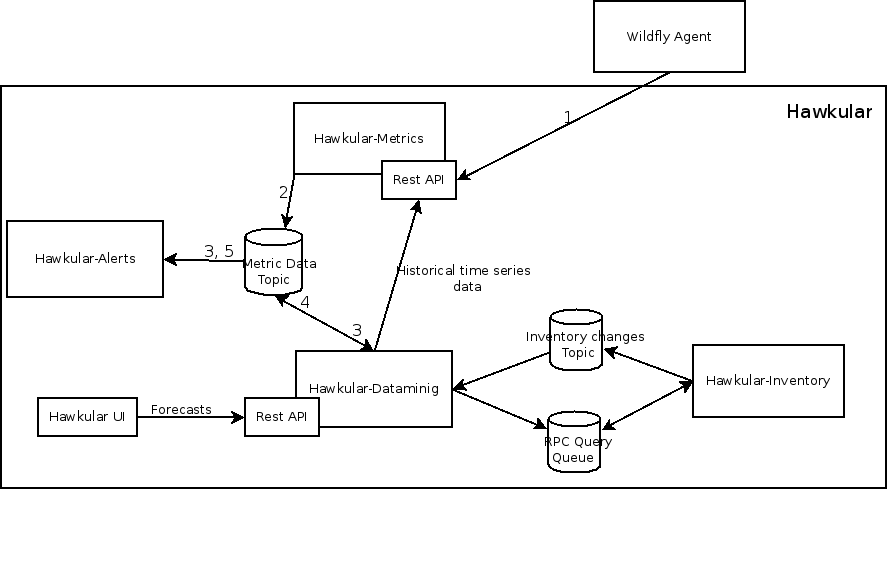
\includegraphics{img/architecture.png}} 
            \caption{The integration with Hawkular.}
            \label{img_integration}
        \end{center}
    \end{figure}

    %%%%%%%%
    \section{Design of data structures}
    In this section are described the most interesting parts of the implementation.
    
    Hawkular Inventory stores all entities of the application. Back end is graph
    database\footnote{Compatible with Apache Tinkerpop\,--\,Titan and TinkerGraph}.
    In the \ref{img_inventory} is showed part of the entities which are important for 
    Data mining module.
    Intentory high level API offers creating relationships between arbitrary entities. 
    This was used for enabling forecasting. This relationship contains properties map
    where is stored configuration of forecasting.

    \begin{figure}[H]
        \begin{center}
            \scalebox{0.5}{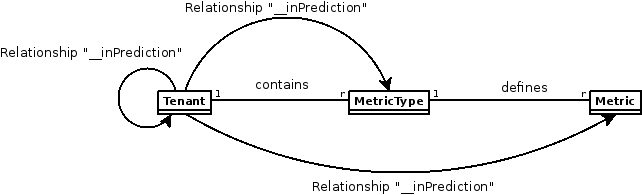
\includegraphics{img/inventory.png}} 
            \caption{Structure of Inventory.}
            \label{img_inventory}
        \end{center}
    \end{figure}

    For subscribing predictions and holding models was designed interface
    \texttt{ModelManager} \ref{alg_modelManager}. 
    Implementation of this interface holds in memory 
    objects of models with respect to hierarchy of Inventory.

    \begin{lstlisting}[caption={Interface Model Manager}, language=Java, label={alg_modelManager}]
     public interface ModelManager {
         void subscribe(Metric, Set<ModelOwner>);
         void unSubscribe(tenantId, metricId);
         Model model(tenantId, metricId);
         ...
     }
    \end{lstlisting}

    \texttt{ModelManager} is initialized on application startup and any change in
    Inventory is propagated through JMS to this object. With this approach Data mining is
    always synchronized with inventory. 

    Interface \texttt{ForecastingEngine} \ref{alg_forecaEngine} provides forecasts for
    subscribed metrics. Implementation of this interface contains \texttt{ModelManager}.
    
    \begin{lstlisting}[caption={Interface Forecasting Engine}, language=Java, label={alg_forecaEngine}]
     public interface ForecastingEngine {
         void learn(List<DataPoint> ts);
         void List<DataPoint> predict(tenantId, metricId, nAhead);
         ...
     }
    \end{lstlisting}

    %%%%%%%%
    \section{Testing and Documentation}
    Unit tests were developed to cover crucial functionality of the program. The
    frameworks JUnit and TestNG are used for testing. Data mining module interacts with many other modules so
    integration and end to end tests were also implemented. Integration and end to end
    tests were written in Groovy because of the simple and well-arranged http client. It
    is also possible to easy define JSON string which is sent as POST object.

    Documentation is written directly in Java code as javadoc. Documentation of the REST
    API was automatically generated by framework Swagger\footnote{Available at
    \url{http://swagger.io/}} and then automatically uploaded at Hawkular website. This
    was done at every build in Travis-CI. With this approach there were always the newest 
    documentation available.

%%%%%%%%%%%%%%%%%%%%%%%%%%%%%%%%%%%%%%%%%%%%%%%%%%%%%%%%%%%%%%%%%%% 
\chapter{Evaluation}
%TODO
TODO do an example how to generate an alert.
maybe generate synthetic data and use it as input for models.

    %%%%%%%% 
    \section{The Most Important Metrics}
    %TODO 
    TODO select subset of the most important metrics and show on them predictions.

%%%%%%%%%%%%%%%%%%%%%%%%%%%%%%%%%%%%%%%%%%%%%%%%%%%%%%%%%%%%%%%%%%% 
\chapter{Conclusion}

